\documentclass{standalone}
\usepackage{tikz}
\usetikzlibrary{patterns, positioning}


\begin{document}
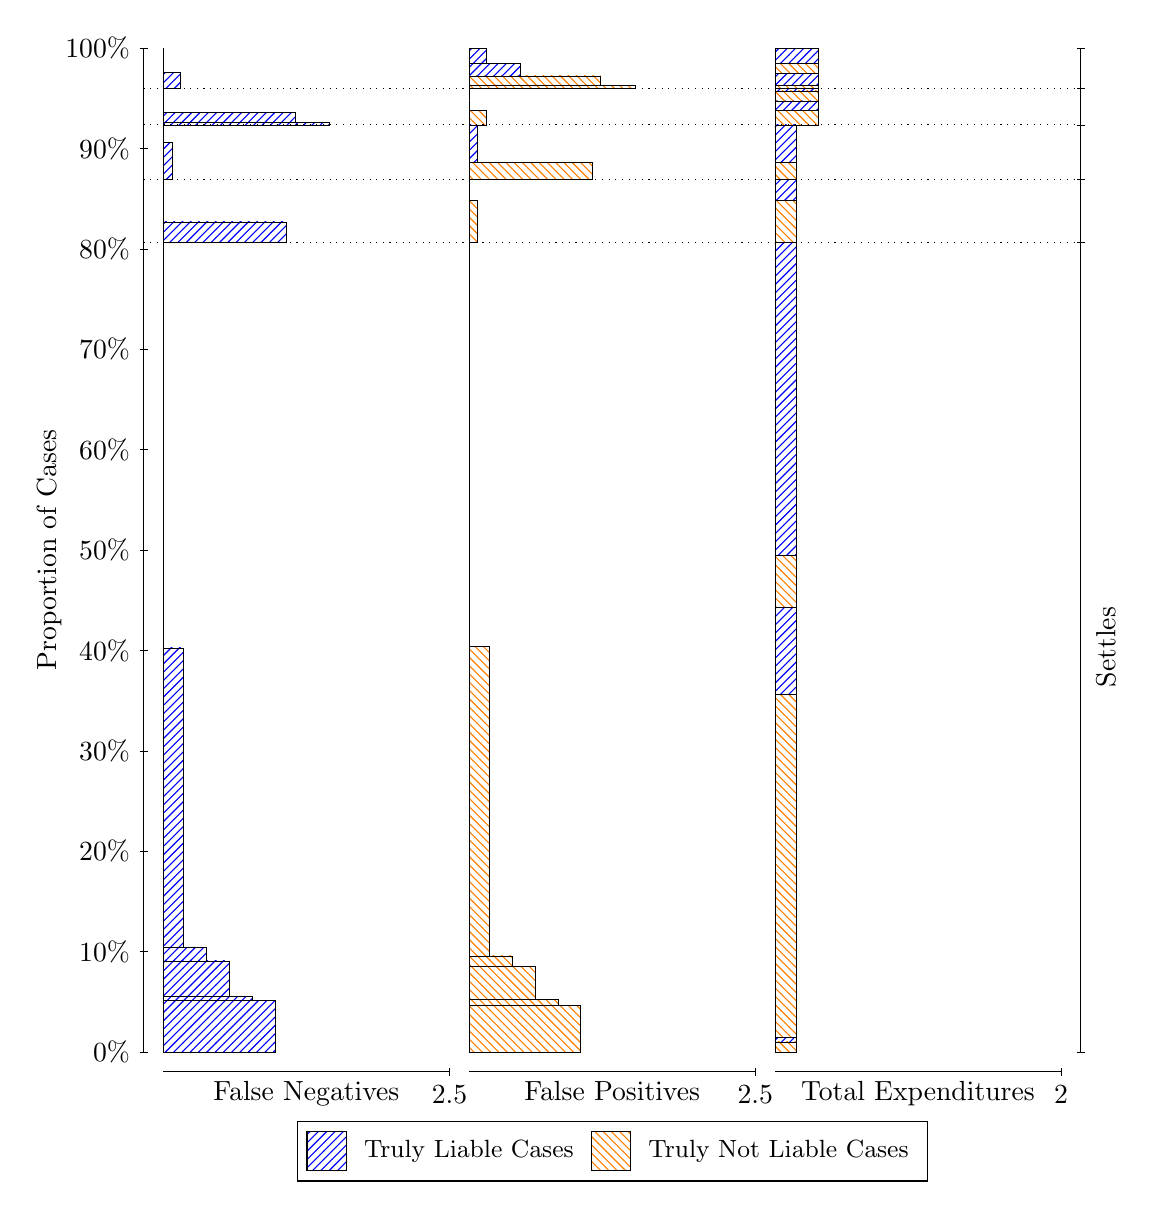
\begin{tikzpicture}
\draw[black, very thin] (1.5,1.75) -- (1.5,14.5);
\node[rotate=90, text=black, anchor=center] at (0.3, 8.125) {Proportion of Cases};
\draw[black, very thin] (1.45,1.75) -- (1.55,1.75);
\node[text=black, anchor=east] at (1.45, 1.75) {0\%};
\draw[black, very thin] (1.45,3.025) -- (1.55,3.025);
\node[text=black, anchor=east] at (1.45, 3.025) {10\%};
\draw[black, very thin] (1.45,4.3) -- (1.55,4.3);
\node[text=black, anchor=east] at (1.45, 4.3) {20\%};
\draw[black, very thin] (1.45,5.575) -- (1.55,5.575);
\node[text=black, anchor=east] at (1.45, 5.575) {30\%};
\draw[black, very thin] (1.45,6.85) -- (1.55,6.85);
\node[text=black, anchor=east] at (1.45, 6.85) {40\%};
\draw[black, very thin] (1.45,8.125) -- (1.55,8.125);
\node[text=black, anchor=east] at (1.45, 8.125) {50\%};
\draw[black, very thin] (1.45,9.4) -- (1.55,9.4);
\node[text=black, anchor=east] at (1.45, 9.4) {60\%};
\draw[black, very thin] (1.45,10.675) -- (1.55,10.675);
\node[text=black, anchor=east] at (1.45, 10.675) {70\%};
\draw[black, very thin] (1.45,11.95) -- (1.55,11.95);
\node[text=black, anchor=east] at (1.45, 11.95) {80\%};
\draw[black, very thin] (1.45,13.225) -- (1.55,13.225);
\node[text=black, anchor=east] at (1.45, 13.225) {90\%};
\draw[black, very thin] (1.45,14.5) -- (1.55,14.5);
\node[text=black, anchor=east] at (1.45, 14.5) {100\%};

\draw[black, very thin] (13.4,1.75) -- (13.4,14.5);
\draw[black, very thin] (13.35,1.75) -- (13.45,1.75);
\node[anchor=west] at (13.35, 1.75) {};
\draw[black, very thin] (13.35,12.034) -- (13.45,12.034);
\node[anchor=west] at (13.35, 12.034) {};
\draw[black, very thin] (13.35,12.827) -- (13.45,12.827);
\node[anchor=west] at (13.35, 12.827) {};
\draw[black, very thin] (13.35,13.525) -- (13.45,13.525);
\node[anchor=west] at (13.35, 13.525) {};
\draw[black, very thin] (13.35,13.99) -- (13.45,13.99);
\node[anchor=west] at (13.35, 13.99) {};
\draw[black, very thin] (13.35,14.5) -- (13.45,14.5);
\node[anchor=west] at (13.35, 14.5) {};

\draw[black, very thin, pattern color=blue, pattern=north east lines] (1.75,1.75) rectangle (3.167,2.405);
\draw[black, very thin, pattern color=blue, pattern=north east lines] (1.75,2.405) rectangle (2.8763,2.4576);
\draw[black, very thin, pattern color=blue, pattern=north east lines] (1.75,2.4576) rectangle (2.5857,2.9057);
\draw[black, very thin, pattern color=blue, pattern=north east lines] (1.75,2.9057) rectangle (2.295,3.0815);
\draw[black, very thin, pattern color=blue, pattern=north east lines] (1.75,3.0815) rectangle (2.0043,6.8807);
\draw[black, very thin, pattern color=orange, pattern=north west lines] (1.75,6.8807) rectangle (1.75,12.034);
\draw[black, very thin, pattern color=blue, pattern=north east lines] (1.75,12.034) rectangle (3.3123,12.293);
\draw[black, very thin, pattern color=orange, pattern=north west lines] (1.75,12.293) rectangle (1.75,12.827);
\draw[black, very thin, pattern color=blue, pattern=north east lines] (1.75,12.827) rectangle (1.859,13.302);
\draw[black, very thin, pattern color=orange, pattern=north west lines] (1.75,13.302) rectangle (1.75,13.525);
\draw[black, very thin, pattern color=blue, pattern=north east lines] (1.75,13.525) rectangle (3.8573,13.56);
\draw[black, very thin, pattern color=blue, pattern=north east lines] (1.75,13.56) rectangle (3.4213,13.683);
\draw[black, very thin, pattern color=orange, pattern=north west lines] (1.75,13.683) rectangle (1.75,13.99);
\draw[black, very thin, pattern color=blue, pattern=north east lines] (1.75,13.99) rectangle (1.968,14.19);
\draw[black, very thin, pattern color=orange, pattern=north west lines] (1.75,14.19) rectangle (1.75,14.347);
\draw[black, very thin, pattern color=blue, pattern=north east lines] (1.75,14.347) rectangle (1.75,14.5);
\draw[black, very thin, pattern color=orange, pattern=north west lines] (5.6333,1.75) rectangle (7.0503,2.3464);
\draw[black, very thin, pattern color=orange, pattern=north west lines] (5.6333,2.3464) rectangle (6.7597,2.4162);
\draw[black, very thin, pattern color=orange, pattern=north west lines] (5.6333,2.4162) rectangle (6.469,2.8418);
\draw[black, very thin, pattern color=orange, pattern=north west lines] (5.6333,2.8418) rectangle (6.1783,2.9699);
\draw[black, very thin, pattern color=orange, pattern=north west lines] (5.6333,2.9699) rectangle (5.8877,6.9034);
\draw[black, very thin, pattern color=blue, pattern=north east lines] (5.6333,6.9034) rectangle (5.6333,12.034);
\draw[black, very thin, pattern color=orange, pattern=north west lines] (5.6333,12.034) rectangle (5.7423,12.568);
\draw[black, very thin, pattern color=blue, pattern=north east lines] (5.6333,12.568) rectangle (5.6333,12.827);
\draw[black, very thin, pattern color=orange, pattern=north west lines] (5.6333,12.827) rectangle (7.1957,13.05);
\draw[black, very thin, pattern color=blue, pattern=north east lines] (5.6333,13.05) rectangle (5.7423,13.525);
\draw[black, very thin, pattern color=orange, pattern=north west lines] (5.6333,13.525) rectangle (5.8513,13.705);
\draw[black, very thin, pattern color=orange, pattern=north west lines] (5.6333,13.705) rectangle (5.6333,13.833);
\draw[black, very thin, pattern color=blue, pattern=north east lines] (5.6333,13.833) rectangle (5.6333,13.99);
\draw[black, very thin, pattern color=orange, pattern=north west lines] (5.6333,13.99) rectangle (7.7407,14.027);
\draw[black, very thin, pattern color=orange, pattern=north west lines] (5.6333,14.027) rectangle (7.3047,14.147);
\draw[black, very thin, pattern color=blue, pattern=north east lines] (5.6333,14.147) rectangle (6.2873,14.3);
\draw[black, very thin, pattern color=blue, pattern=north east lines] (5.6333,14.3) rectangle (5.8513,14.5);
\draw[black, very thin, pattern color=orange, pattern=north west lines] (9.5167,1.75) rectangle (9.7892,1.8782);
\draw[black, very thin, pattern color=blue, pattern=north east lines] (9.5167,1.8782) rectangle (9.7892,1.9308);
\draw[black, very thin, pattern color=orange, pattern=north west lines] (9.5167,1.9308) rectangle (9.7892,6.2898);
\draw[black, very thin, pattern color=blue, pattern=north east lines] (9.5167,6.2898) rectangle (9.7892,7.3928);
\draw[black, very thin, pattern color=orange, pattern=north west lines] (9.5167,7.3928) rectangle (9.7892,8.059);
\draw[black, very thin, pattern color=blue, pattern=north east lines] (9.5167,8.059) rectangle (9.7892,12.034);
\draw[black, very thin, pattern color=orange, pattern=north west lines] (9.5167,12.034) rectangle (9.7892,12.568);
\draw[black, very thin, pattern color=blue, pattern=north east lines] (9.5167,12.568) rectangle (9.7892,12.827);
\draw[black, very thin, pattern color=orange, pattern=north west lines] (9.5167,12.827) rectangle (9.7892,13.05);
\draw[black, very thin, pattern color=blue, pattern=north east lines] (9.5167,13.05) rectangle (9.7892,13.525);
\draw[black, very thin, pattern color=orange, pattern=north west lines] (9.5167,13.525) rectangle (10.062,13.705);
\draw[black, very thin, pattern color=blue, pattern=north east lines] (9.5167,13.705) rectangle (10.062,13.828);
\draw[black, very thin, pattern color=orange, pattern=north west lines] (9.5167,13.828) rectangle (10.062,13.955);
\draw[black, very thin, pattern color=blue, pattern=north east lines] (9.5167,13.955) rectangle (10.062,13.99);
\draw[black, very thin, pattern color=orange, pattern=north west lines] (9.5167,13.99) rectangle (10.062,14.027);
\draw[black, very thin, pattern color=blue, pattern=north east lines] (9.5167,14.027) rectangle (10.062,14.18);
\draw[black, very thin, pattern color=orange, pattern=north west lines] (9.5167,14.18) rectangle (10.062,14.3);
\draw[black, very thin, pattern color=blue, pattern=north east lines] (9.5167,14.3) rectangle (10.062,14.5);
\draw[black, dotted] (1.5,12.034) -- (13.4,12.034);
\draw[black, dotted] (1.5,12.827) -- (13.4,12.827);
\draw[black, dotted] (1.5,13.525) -- (13.4,13.525);
\draw[black, dotted] (1.5,13.99) -- (13.4,13.99);
\draw[black, very thin] (1.75,1.5) -- (5.3833,1.5);
\node[text=black, anchor=north] at (3.5667, 1.5) {False Negatives};
\draw[black, very thin] (5.3833,1.45) -- (5.3833,1.55);
\node[text=black, anchor=north] at (5.3833, 1.45) {2.5};

\draw[black, very thin] (5.6333,1.5) -- (9.2667,1.5);
\node[text=black, anchor=north] at (7.45, 1.5) {False Positives};
\draw[black, very thin] (9.2667,1.45) -- (9.2667,1.55);
\node[text=black, anchor=north] at (9.2667, 1.45) {2.5};

\draw[black, very thin] (9.5167,1.5) -- (13.15,1.5);
\node[text=black, anchor=north] at (11.333, 1.5) {Total Expenditures};
\draw[black, very thin] (13.15,1.45) -- (13.15,1.55);
\node[text=black, anchor=north] at (13.15, 1.45) {2};

\node[text=black, centered, rotate=90] at (13.72, 6.892) {Settles};





\draw (7.449999999999999,1.5) node[draw=none] (baseCoordinate) {};
\begin{scope}[align=center]
        \matrix[scale=0.5, draw=black, below=0.5cm of baseCoordinate, nodes={draw}, column sep=0.1cm]{
            \node[rectangle, draw, minimum width=0.5cm, minimum height=0.5cm, pattern color=blue, pattern=north east lines] {}; &
            \node[draw=none, font=\small, text=black] (B) {Truly Liable Cases}; &
            \node[rectangle, draw, minimum width=0.5cm, minimum height=0.5cm, pattern color=orange, pattern=north west lines] {}; &
            \node[draw=none, font=\small, text=black] (B) {Truly Not Liable Cases}; \\
            };
\end{scope}

\end{tikzpicture}
\end{document}